\part{Implementation}
\chapter{Quanthon: Quantum Computing in Python}
\label{ch:quanthon}

This chapter details the design and implementation of a quantum computing library in Python~\cite{python3}, namely \texttt{Quanthon}. The library can be found at \url{https://pypi.org/project/Quanthon/} and the source code at \url{https://github.com/moyasui/Quanthon}.

While existing quantum computing libraries such as Qiskit~\cite{qiskit}, and Circ~\cite{cirq_2024} are usually better integrated with hardware, more optimised and contain more functionalities, writing an entire library from scratch can be beneficial pedagogically by forbidding the existence of black boxes as well as allowing more freedom in structures and conventions. One example of such is the ordering of qubits. Let $ A, B,C,D $ be single-qubit operations, most literature uses $ ABCD $ to mean $ A_1B_2C_3D_4 $ i.e. applying the gate $ A $ on the first qubit, $ B $ on the second etc. This, however, is inconsistent with the computer science convention of representing numbers using bit strings, where the most significant bit is to the left. For example, the decimal $ 4 $ is usually written as $ 100 $ in binary representation. Most quantum computing libraries adhere to the binary representation convention by having the most significant bit to the left, therefore logically the aforementioned 4-qubit gate should have been written as $ DCBA $, which sadly is not. There is no physical reason for this choice and it is purely conventional, hence no reason to compromise for it. In Quanthon, the most significant bit is to the right, and the order of operators/gates is written normally, in the same order.  

Quanthon is also designed to be minimalistic and with the focus of physicists in mind. The library is designed to be used for quantum simulations and solving physical problems, following the most fundamental principles rather than specialising in, e.g.\ electronic systems. The library is also designed to be easily extensible, with the ability to add custom gates and operators, algorithms and models. 

Quanthon will continue to be maintained and expanded after the conclusion of this master's project. 

\newpage

\section{Architecture}
\label{sec:arch}
\begin{figure}[ht]
	\centering
	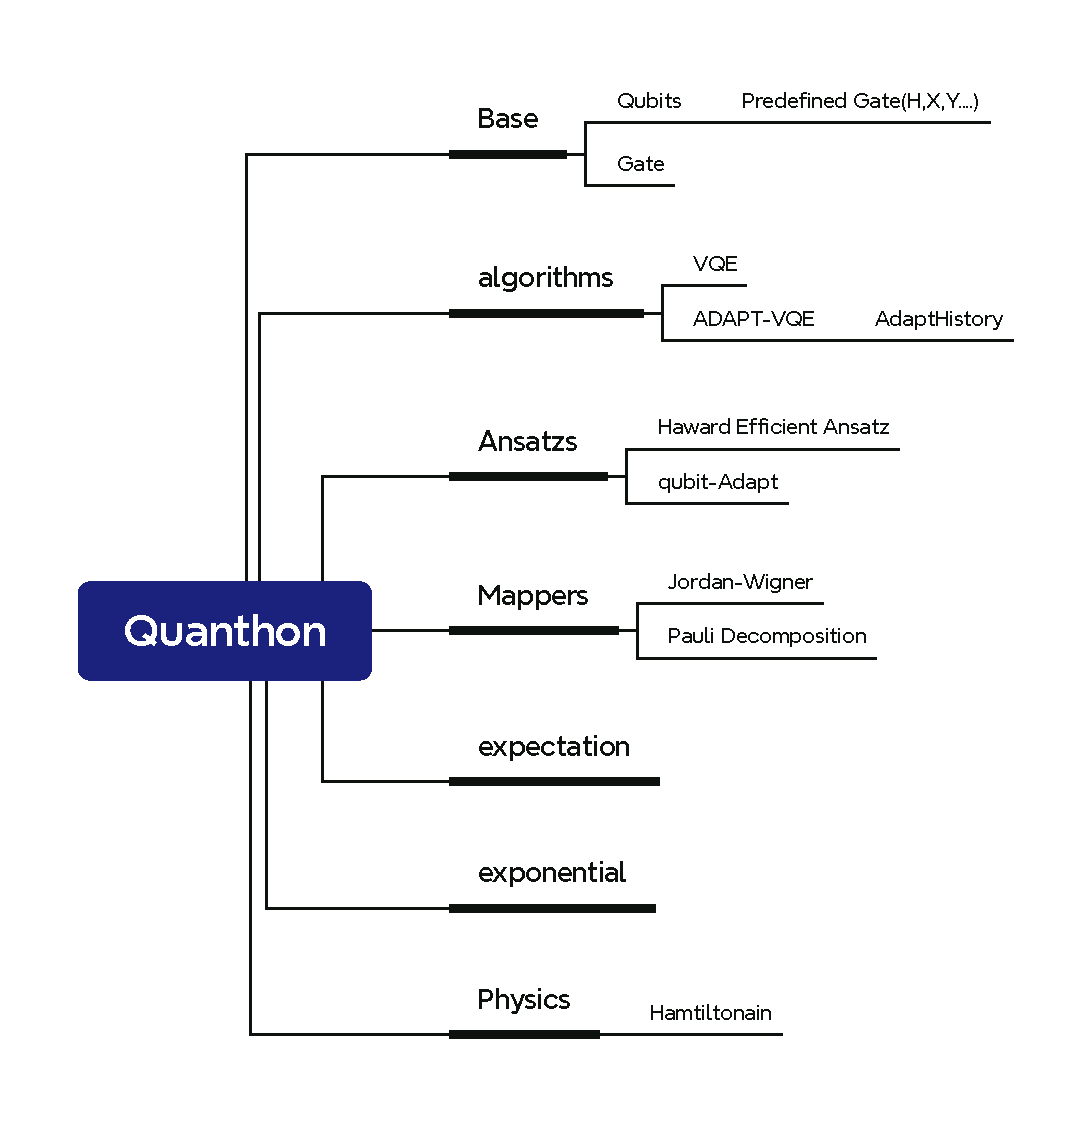
\includegraphics[width=\textwidth]{image/architecture.pdf}
	\caption{Architecture of Quanthon.}
	\label{fig:image-architecture}
\end{figure}

Figure~\ref{fig:image-architecture} shows the architecture of Quanthon. Quanthon is built with quantum simulations and solving physical problems in mind, and it is divided into a few modules and several standalone functions. The basic module is the \texttt{base} module, this is where all the circuitry and gates are defined. The \texttt{algorithms} and \texttt{Ansatz} are heavily focused on the Variational Quantum Eigensolver. The \texttt{expectation} module contains functions that calculate the expectation value of an operator and \texttt{exponential} creates a circuit which exponentiates a Pauli string. The \texttt{Physics} module is used for storing the integrals of a second quantised Hamiltonian. The \texttt{Mappers} contains functions for transforming the Hamiltonian from different forms in terms of Pauli operators. The \texttt{utils} and \texttt{mappers\_utils} modules contain helper functions.

\newpage
\section{Basic Elements of Quantum Computing}
\label{sec:base}
In theory, all quantum computation can be simulated using only these basic elements we introduce in this section, qubits and gates as described in Chapter~\ref{ch:qc}. 
This section explains the structure for \texttt{base.py}, including the \texttt{Gate} class and \texttt{Qubits} class.
\subsection{Qubits}
\label{sub:qubits}
A \texttt{Qubits} object is the most fundamental unit for quantum computation. It contains information about
\begin{itemize}
	\item the number of qubits, \texttt{Qubits.n\_qubit},
	\item the current circuit, \texttt{Qubits.circuit},
	\item the current state of the qubits, \texttt{Qubits.state},
	\item the history of all the gates applied to the circuit, which is not cleared when the circuit is reset \texttt{Qubits.gate\_history},.
\end{itemize}

Initialise a \texttt{Qubits} object of $ 2 $ qubits to the $ \ket{0} $ state by calling
\begin{mycode}
	from Quanthon import Qubits
	q = Qubits(2)
\end{mycode}
 

To manipulate the circuit by appending gates to the circuit,
\begin{mycode}
	q.H(0) # appends the Hadamard gate (a \texttt{Gate} object) on the $ 0th $ qubit to q.circuit. \
	q.CNOT(0,1) # appends the CNOT with control qubit $ 0 $  and target qubit $ 1 $ to q.circuit. \
	q.run() # apply all the gates in q.circuit
	q.draw() # generate code for drawing the circuit in Quantikz~\cite{kay2023tutorialquantikzpackage}.
\end{mycode}
Below we list all currently available gates as methods of the \texttt{Qubits} class
\begin{itemize}
	\item \texttt{H} (Hadamard gate), 
	\item \texttt{X,Y,Z} (Pauli matrices),
	\item \texttt{Rx, Ry, Rz} (single qubit rotation gates),
	\item \texttt{Sdag}, $ S^{\dagger}$, the Hermitian conjugate of the S-phase gate,
	\item  \texttt{CNOT} (controlled-not) gate,
	\item \texttt{SWAP} (the swap gate).
\end{itemize}
To simulate a classical measurement with $ n $ shots, where the probability is given by amplitude squared using the Born rule.
\begin{mycode}
	counts = q.measure(n_shots=10000)
\end{mycode}
where \texttt{count} contains the simulated result for $ 10000 $ shots of the same circuit \texttt{q}. The output is a $ 2^n \times 2 $ array, the first column is the count corresponding to the state in binary in the second column.

\begin{mycode}
>>> counts
array([[5025, '00'],
       [0, '01'],
       [0, '10'],
       [4975, '11']], dtype=object)
\end{mycode}
Other available methods that could be useful include
\begin{itemize}
	\item \texttt{reset} to reset the state of the qubits to $ \ket{0} $,
	\item \texttt{set\_state} which sets the state of the qubits to a given state, also checks if the state is valid,
	\item \texttt{reset\_circuit} which resets the circuit to an empty list,
	\item \texttt{copy} which returns a copy of the \texttt{Qubits} object with the same states but not gates in the circuit, this is useful when repeated circuit preparation is needed for measurement,
	\item \texttt{\_to\_comp\_basis} which returns the state in the more readable bra-ket notation when the print statement is called. For example, the following code gives
\begin{mycode}
	>>> q = Qubits(2)
	>>> print(q)	
\end{mycode} 
	\[ \text{Qubit(s) in state:} 1.00+0.00j\ket{00} \]
	\item \texttt{count\_gates} which returns the length of the circuit
	\item \texttt{count\_cnots} which returns the number \cnot gates currently in the circuit.
	\texttt{draw} provides visualisation of the circuit and returns a Quantikz \missingref string that represents the circuit.
\end{itemize}


\subsection{Shot Noise}%
\label{sub:shot_noise}
In this section, we will numerically show the error of state tomography for different numbers of shots and compare their precisions. We first prepare a state $ \ket{\psi}  $ such that
\[ \ket{\psi} = \frac{1}{2} \left( \ket{00} + \ket{01} + \ket{10} + \ket{11} \right)  \] 
We now measure the state $ \ket{\psi} $ for $ [4^2, 4^3, 4^4, 4^5, 4^6, 4^7, 4^8, 4^9]$ shots and compare the error, as well as to the theoretical result from Subsection~\ref{sub:measurement}. If the precision required is $ \epsilon $ then the number of shots required $ \propto \frac{1}{\epsilon^2} $. Then every time the number of shots is increased by a factor of four, the error should be reduced by a factor of $\frac{1}{2}$. 
\begin{figure}[ht]
	\centering
	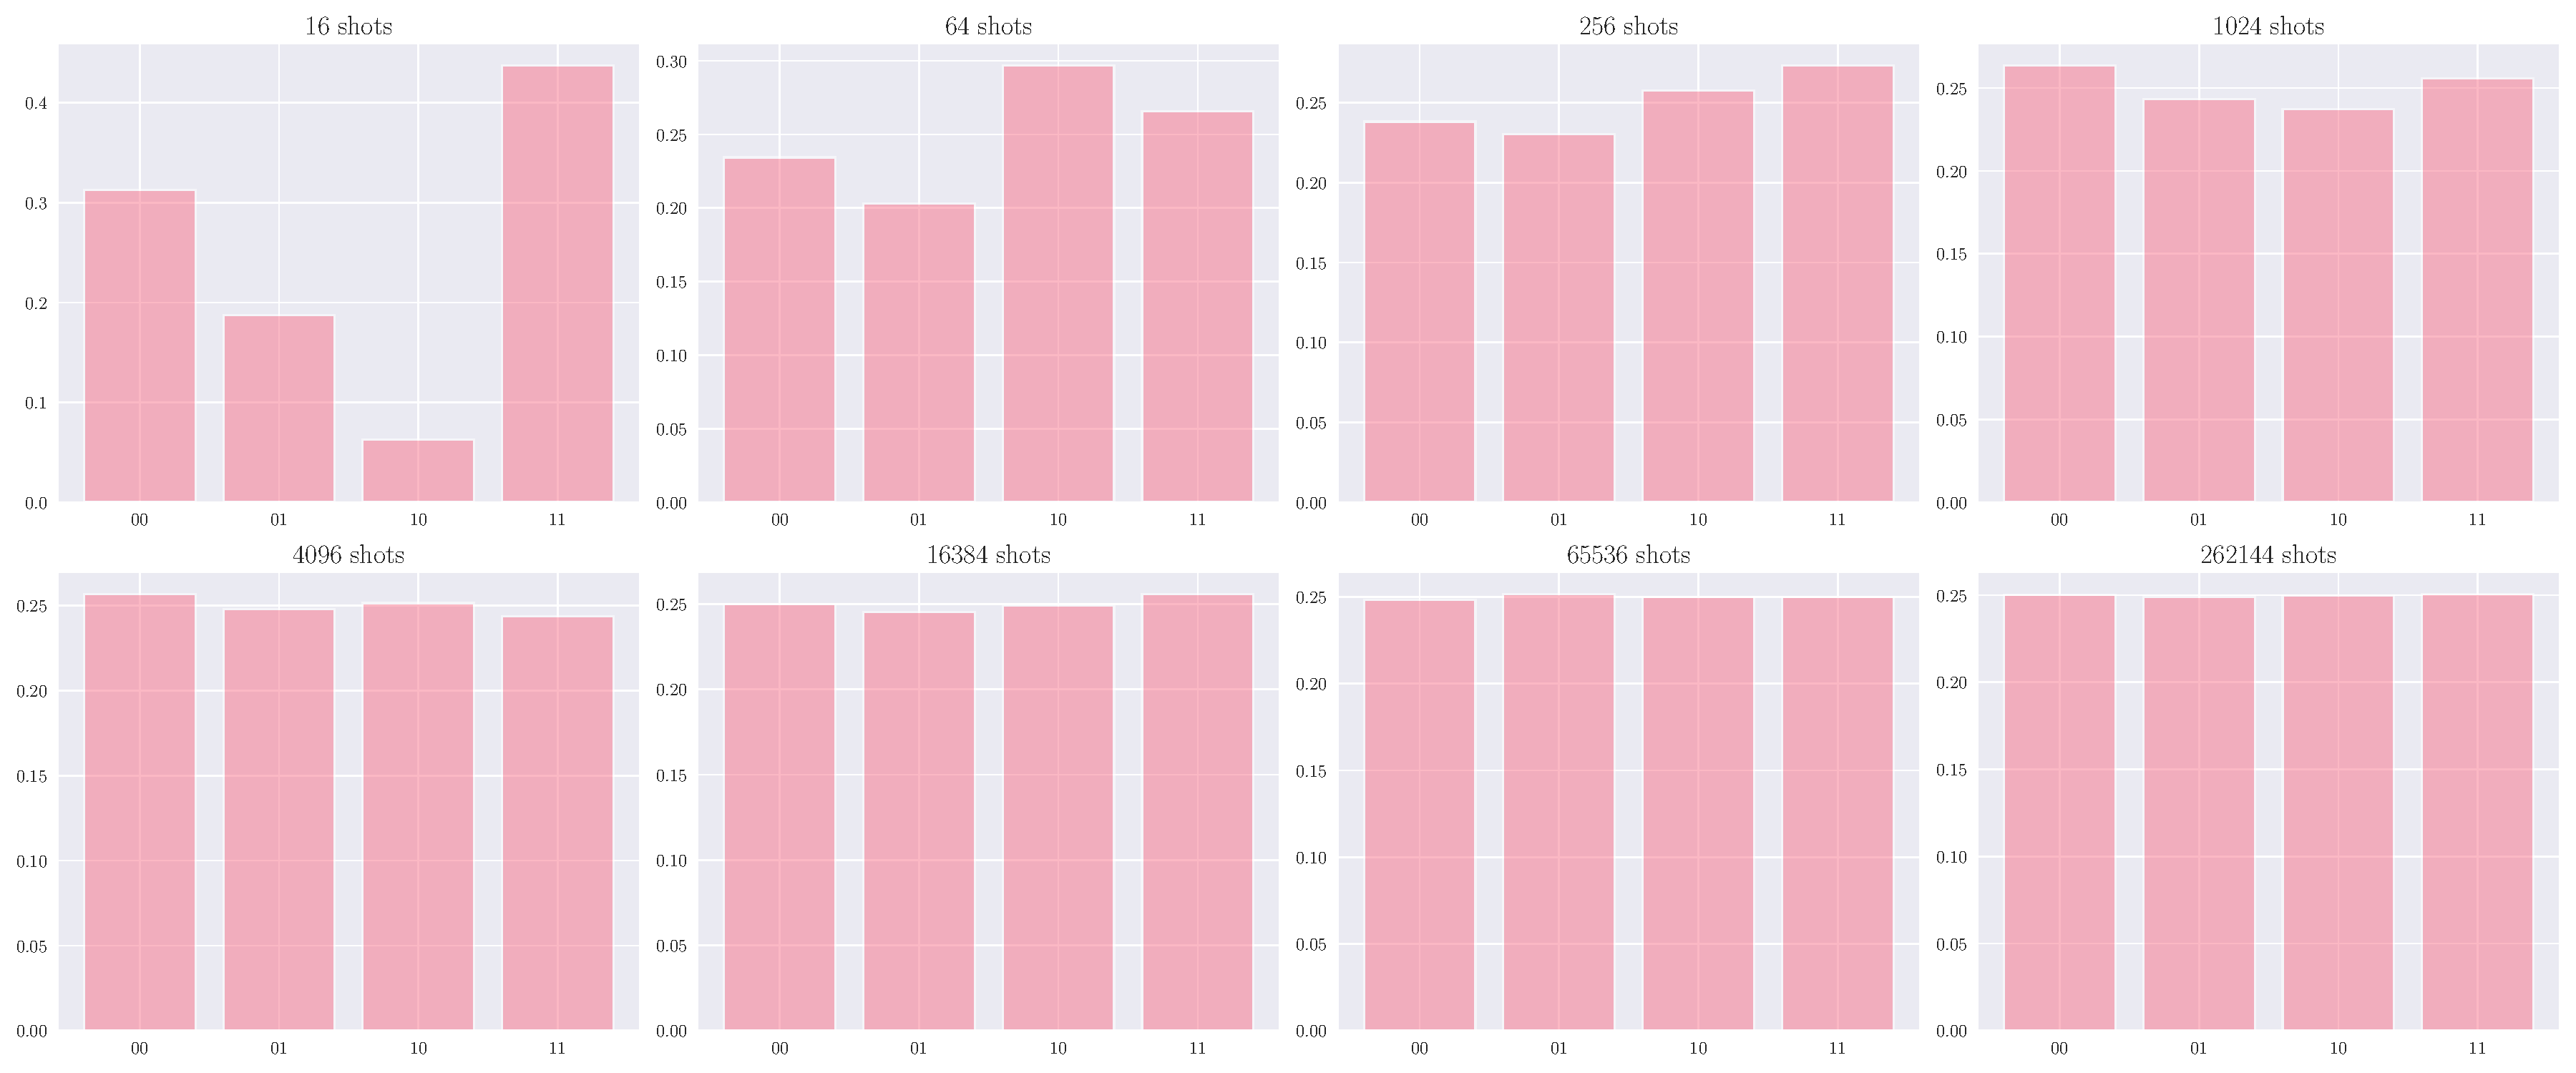
\includegraphics[width=\linewidth]{image/measurements_histogram.pdf}
	\caption{Histograms of classically simulated measurement results for state $\ket{\psi} $ with different number of shots. The horizontal axis labels the states being measured and the vertical axis shows the probability for measuring the corresponding state.}
	\label{fig:meas_result}
\end{figure}


\begin{figure}[ht]
	\centering
	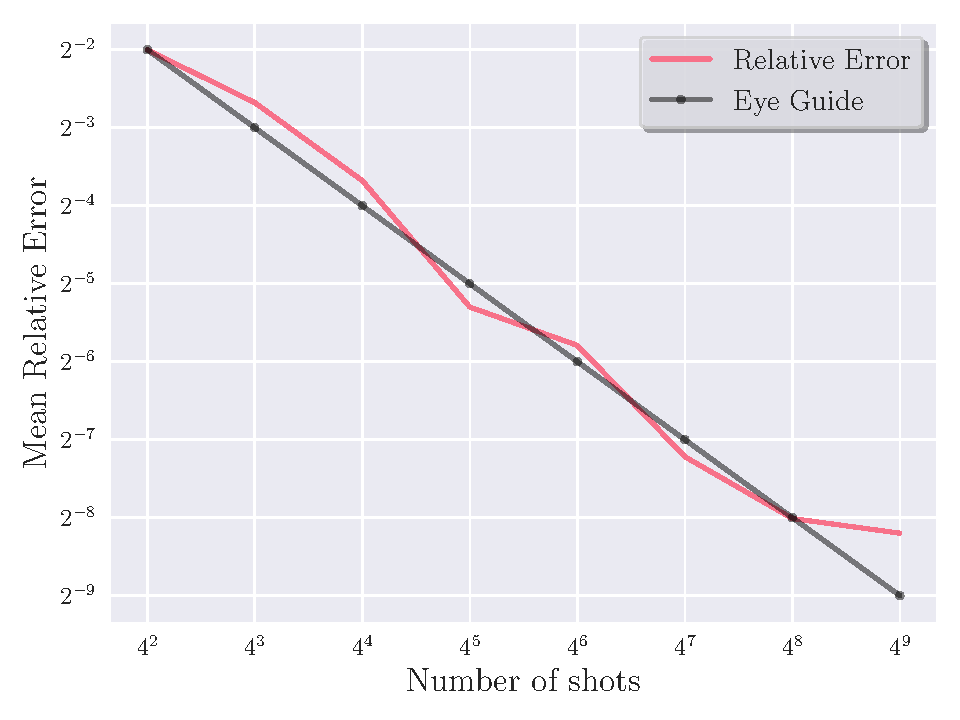
\includegraphics[width=0.8\linewidth]{image/mean_rel_error.pdf}
	\caption{Mean relative error for each shot. The red line is the result of a numerical simulation using the \texttt{Quanthon} library and the grey line is an eye guide with $ y = 1/\sqrt{x} $.}
	\label{fig:mean_rel_err}
\end{figure}

Figures~\ref{fig:meas_result} and ~\ref{fig:mean_rel_err} demonstrate the relationship between the error and the number of shots we see that the results agree quite well with the theoretical result: $ N \propto \mathcal{O}(\frac{1}{ \epsilon^2 }) $. In fact, from Figure~\ref{fig:mean_rel_err} we can estimate errors from measurements with $ \epsilon \propto \sqrt{\frac{1}{N}} $. Later we will show that the error from shot noise is the limiting factor for the accuracy of algorithms. 


\subsection{Gate}
\label{sub:gate}
The \texttt{Qubits} class contains common predefined gates as in Subsection~\ref{sub:qubits}.
To construct a custom gate, which can be parameterised, specify the name, the number of qubits being acted on and the matrix representation of the gate or a function which takes in parameters and generates the gate matrix. The matrix must be unitary according to Definition~\ref{def:unitary}. \\
Below is an example of how to construct an \texttt{Rz} gate for a two-qubit circuit.
\begin{mycode}
import numpy as np
from Quanthon.base import Gate
from Quanthon.utils import make_op_mat

def Rz(theta, n, i):
	"""
        Args: 
            theta: float, the angle of rotation in radians,
            n: int, the number of qubits in the system,
            i: int, the index to apply the gate to.
        
        Returns:
            mat: the matrix representing the rotation of qubit i by theta about the z-axis.
	"""
    
    rz = np.cos(theta/2)*np.eye(2) - 1j*np.sin(theta/2)*np.array([[0,1],[1,0]])
    mat = make_op_mat(rz, i) # this expands the matrix to the size of the full system
    return mat

n = 2
i = 0
# non-parameterised
theta = 0.5 * np.pi
mat = Rz(theta, n, i)
rz_gate = Gate("Rz", mat, n)

# Parameterised
rz_gate_param = Gate("Rz", lambda theta: Rz(theta,i,n), n, is_parametrised=True)
\end{mycode}

To use the custom gate, 
\begin{mycode}
	q = qubits(2)
	# apply the non-parameterised Rz gate
	q.circuit.append(rz_gate) # append the gate here without any parameter 
	q.run()

	# or the parameterised gate
	q.state = rz_gate_param.act(q.state, 0.5 * np.pi)
	
\end{mycode}
Note that custom gates do not currently support drawing.


\section{Expectation Value}
\label{sec:expectation}
The expectation value of an operator $ A $ is given as 
\[ \braket{\psi|A|\psi}. \]
In a real quantum computer, this value must be estimated through repeated measurements of the state of the qubits on different basis. Since the Pauli matrices together with the identity operator $ I $ form a basis for the $2 \times 2$ matrices ( $\mathcal{M}_{2\times 2}$), any operator in this space can be written in terms of a linear combination of these operators using methods given in Appendix~\ref{appsec:pauli_basis}.

Let $ P $ be a Pauli string, then the expectation value of $ P $ is given by
\begin{equation}
	\label{eq:expectation}
	\braket{\psi|P|\psi} = \braket{\psi|U^{\dagger}ZU|\psi}.
\end{equation}

One must find a unitary operator $ U $ such that $ U^{\dagger}ZU $ is equal to the basis we are trying to measure in the one-qubit case, and $ ZI\ldots I $ in the multiple-qubit case. When the unitary transformation $ U $ is applied to the circuit of which we want to measure the expectation value, the eigenvalues are preserved and the expectation value can be calculated in the new basis.

\subsection{Single Qubit}
\label{sub:single_qubit}
In general, the one qubit Hamiltonian can be written as 
\begin{equation}
	\label{eq:1qubit_hamiltonian}
	H = aI + bX + cY + dZ, \quad a,b,c,d \in \mathbb{C}. 
\end{equation}

Given the following relations relating the Pauli $ X $ and $ Y $ operator with the Pauli $ Z $,
\begin{align}
	\label{eq:basis-rotation}
	X = HZH, \\
	Y = -S^{\dagger}HZHS.
\end{align}

Then the expectation value is 
\begin{align}
	\braket{\psi|H|\psi} &= a\braket{\psi|I|\psi} + b \braket{\psi|X|\psi} + c \braket{\psi|Y|\psi} + d \braket{\psi|Z|\psi} \\
			     &= a \underbrace{\braket{\psi|\psi}}_{1} + b \braket{\psi|HZH|\psi} + c \braket{\psi|HS^{\dagger}ZSH|\psi} + d \braket{\psi|Z|\psi}.
\end{align}

The \texttt{expectation} function estimates the expectation values of a qubit Hamiltonian.

In the case of a single qubit, to rotate the computation basis to another Pauli basis, we simply apply the $H$ gate for when there is an $ X $ in the Hamiltonian, and $ S^\dagger$ gate followed by an $ H $ gate when there is a $ Y $-gate.

\begin{figure}[ht]
	\centering
	\begin{quantikz}
		  & \gate{U} & \gate{H}  &\qw\\
	\end{quantikz}
	\caption{The single qubit circuit which rotates a state to be measured in the $ X $ basis.}
	\label{fig:rotate-to-X-circuit}
\end{figure}

\subsection{Multiple Qubits}
\label{sub:multiple_qubits}
The computation basis is the Pauli $ Z\underbrace{I \ldots I}_{n-1}$ basis for an $ n $-qubit quantum circuit. 
When there is more than one qubit in the system if the operator contains only one non-identity operator on the first qubit, then a similar strategy applies --- apply the \texttt{H}-gate or the \texttt{Sdag}-gate followed by \texttt{H} gate on the first qubit. 

In the case where the Pauli string contains more than non-identity, for example, $ZI$ contains only one non-identity operator and $ZZ$ contains two, the \texttt{CNOT} gate must be applied to such qubits to disentangle them. Consider the smallest non-trivial case, the Pauli string $ ZZ $, the unitary transform which rotates the $ ZZ $ basis to the $ ZI $ basis is the $ CNOT_{10} $ gate,
\[
CNOT(1,0) =
\begin{bmatrix} 
1 & 0 & 0 & 0 \\
0 & 0 & 0 & 1 \\
0 & 0 & 1 & 0 \\
0 & 1 & 0 & 0 \\
\end{bmatrix} = CNOT(1,0)^{\dagger},  \] 
and
\begin{align}
	CNOT(1,0)(ZZ)CNOT(1,0) &= 
\begin{bmatrix} 
1 & 0 & 0 & 0 \\
0 & 0 & 0 & 1 \\
0 & 0 & 1 & 0 \\
0 & 1 & 0 & 0 \\ 
\end{bmatrix} 
\begin{bmatrix} 
1 & 0 & 0 & 0 \\
0 & -1 & 0 & 0 \\
0 & 0 & -1 & 0 \\
0 & 0 & 0 & 1 \\
\end{bmatrix} 
\begin{bmatrix}
1 & 0 & 0 & 0 \\
0 & 0 & 0 & 1 \\
0 & 0 & 1 & 0 \\
0 & 1 & 0 & 0 \\
\end{bmatrix} \\
&= 
\begin{bmatrix}
1 & 0 & 0 & 0 \\
0 & 1 & 0 & 0 \\
0 & 0 & -1 & 0 \\
0 & 0 & 0 & -1 \\
\end{bmatrix} = ZI.
\end{align}


\begin{figure}[ht]
	\centering
	\begin{quantikz}
		\lstick{$\ket{q_1}$} &\gate[2]{U} & \ctrl{1} & \qw \\
		\lstick{$\ket{q_2}$} & \qw & \targ{} & \qw
	\end{quantikz}
	\caption{The circuit to rotate the qubits into the $ ZZ $ basis.}
	\label{fig:disentangle-ZZ}
\end{figure}
In cases where the non-identity gates are not in the first positions, a series of SWAP gates are used to swap the state of the qubits with neighbouring qubits,

\begin{align}
	\label{eq:swap}
	SWAP(0,1)(IZ)SWAP(0,1) &=  
\begin{bmatrix}
1 & 0 & 0 & 0 \\
0 & 0 & 1 & 0 \\
0 & 1 & 0 & 0 \\
0 & 0 & 0 & 1 \\
\end{bmatrix}
\begin{bmatrix}
1 & 0 & 0 & 0 \\
0 & -1 & 0 & 0 \\
0 & 0 & 1 & 0 \\
0 & 0 & 0 & -1 \\
\end{bmatrix}
\begin{bmatrix}
1 & 0 & 0 & 0 \\
0 & 0 & 1 & 0 \\
0 & 1 & 0 & 0 \\
0 & 0 & 0 & 1 \\
\end{bmatrix} \\
&=
\begin{bmatrix}
1 & 0 & 0 & 0 \\
0 & 1 & 0 & 0 \\
0 & 0 & -1 & 0 \\
0 & 0 & 0 & -1 \\
\end{bmatrix} = ZI.
\end{align}
\begin{figure}[ht]
	\centering
	\begin{quantikz}
		\lstick{$\ket{q_1}$} &\gate[2]{U} & \swap{1} & \qw \\
		\lstick{$\ket{q_2}$} & \qw & \targX{} & \qw
	\end{quantikz}
	\caption{The circuit to rotate the qubits into the $ IZ $ basis.}
	\label{fig:swap-iz=zi}
\end{figure}

After the rotation, multiple measurements are taken to estimate the state of the qubits, since the eigenvalues are preserved under unitary transformations, the eigenvalues are the same as that of the $ ZI\ldots I $ state. For an $ n $ qubit system, the states $ \ket{0}  $ to $ \ket{2^{n-1}} $ have eigenvalues $ 1 $ and the rest have eigenvalues $ -1 $.

The \texttt{expectation} function handles all the procedures above for all combinations of Pauli strings.  The code snippet outlines the usage of the function.
\begin{mycode}
	from Quanthon import expectation
	q = Qubits(2)
	H = [("ZZ", 0.5), ("XI", 0.5)] # example Hamiltonian, must be given in [(operator, coefficient), ...] format.
	energy = cal_expectation(q, hamiltonian, n_shots=10000)
\end{mycode}


\section{Physics}
\label{sec:physics}
\subsection{Hamiltonian}
The \texttt{Hamiltonian} class stores the overlap integrals for one and two-body. These integrals need to have been calculated. In the case of molecular systems, these integrals can usually be obtained through quantum chemistry packages such as \texttt{PySCF}\cite{sun2018}.

\section{Mappers}
\label{sec:mappers}
\subsection{Jordan-Wigner}
\label{sub:jordan-wigner-mapper}
The Jordan-Wigner transformation maps the fermionic operators to qubit operators. The transformation is given in Section~\ref{sub:jw}.

The second quantised Hamiltonians are usually in the form of Equation~\eqref{eq:sq_hamiltonian}. We keep the integrals general without considering the symmetry of the system, i.e., $ p,q,r,s \in [0, N-1] $ for $ N $ basis functions for both the one- and two-body integrals. The mapping costs $ N $ qubits. The treatment depends on the value and order of the indices and whether it is a one- or two-body term.
\subsection{One-Body}
\label{sub:one-body}
The transformation of the one-body term $ a_{p}^{\dagger}a_q $using Equation~\eqref{eq:jw} is

\begin{equation}
	\label{eq:ob_jw}
a_{p}^{\dagger}a_q \\
				   = \left( \frac{1}{2} \left[ \bigotimes_{n=0}^{p-1} Z_n \right] \left( X_p - i Y_p \right)   \right) 
 \left( \frac{1}{2} \left[ \bigotimes_{n=0}^{q-1} Z_n \right] \left( X_q +i Y_q \right)   \right).
\end{equation}

Four relations are useful in the derivation of the later expressions:
\begin{align}
	\label{eq:useful_relations}
	(X-iY)Z &= -iY+X = (X-iY), \\
	Z(X-iY) &= iY - X = -(X-iY), \\
	(X+iY)Z &= -iY -X = -(X+iY),\\
	Z(X+iY) &= iY + X = (X+iY).
\end{align}

\subsubsection{For $p=q$}%
\label{ssub:p_equal_q}
When $p=q$, using properties of Pauli matrices in Appendix~\ref{app:pauli_properties}, the Jordan-Wigner transform of the term in Equation~\eqref{eq:ob_jw} becomes:
\begin{equation}
	\label{eq:p_equals_q}
	\begin{aligned}
		a_{p}^{\dagger}a_q &= a_{p}^{\dagger}a_p,  \\
				   &= \left( \frac{1}{2} \left[ \bigotimes_{n=0}^{p-1} Z_n \right] \left( X_p - i Y_p \right)   \right) 
 \left( \frac{1}{2} \left[ \bigotimes_{n=0}^{p-1} Z_n \right] \left( X_p +i Y_p \right)   \right), \\
				   &= \frac{1}{4} \left[ \bigotimes_{n=0}^{p-1} I_n \right] \left( X_p - i Y_p \right) \left( X_p + i Y_p \right),\\ 
	&= \frac{1}{4} \left[ \bigotimes_{n=0}^{p-1} I_n \right] \left( X_p^2 -iY_iX_i + iX_iY_i + Y_p^2 \right), \\
	&= \frac{1}{4} \left[ \bigotimes_{n=0}^{p-1} I_n \right] \left( 2I_p + 2iZ_p \right), \\
	&= \frac{1}{2} \left[ \bigotimes_{n=0}^{p-1} I_n \right] \left( I_p -Z_p \right),
	\end{aligned}
\end{equation}
which translates to two Pauli strings. In the case of $ N $ qubits $\underbrace{I\ldots I}_N$ and $\underbrace{I\ldots I}_{p}Z_p \underbrace{l \ldots I}_{N-p-1}$ respectively.


\subsubsection{For $p < q$}%
\label{ssub:p_lessthan_q}
In the case where $ p < q $, the $ Z $ operators on qubits on $ p $ and between $ p $ and $ q $ do not cancel out as in the $ p=q $ case, Equation~\eqref{eq:ob_jw} becomes:
\begin{equation}
	\label{eq:jw_p_lessthan_q}
	\begin{aligned}
		&= \frac{1}{4} \left[ \bigotimes_{n=0}^{p-1} I_n \right] \left( X_p - i Y_p \right)Z_p 
		\left[ \bigotimes_{n=p+1}^{q-1} Z_n \right]  \left( X_q + i Y_q \right) \\
		&= \frac{1}{4} \left[ \bigotimes_{n=0}^{p-1} I_n \right] \left( X_p - i Y_p \right) \left[ \bigotimes_{n=p+1}^{q-1} Z_n \right]  \left( X_q + i Y_q \right) \\
		&= \frac{1}{4} \left[ \bigotimes_{n=0}^{p-1} I_n \right] \left[ \bigotimes_{n=p+1}^{q-1} Z_n \right] \left( X_p - i Y_p \right)   \left( X_q + i Y_q \right) \\
		&= \frac{1}{4} \left[ \bigotimes_{n=0}^{p-1} I_n \right] \left[ \bigotimes_{n=p+1}^{q-1} Z_n \right] \left( X_pX_q - iY_pX_q + iX_pY_q + Y_pY_q \right). \\
	\end{aligned} 
\end{equation}
This translates to four Pauli strings:
\begin{align}
	\label{eq:p_lessthan_q}
	&\underbrace{I\ldots I}_{p}X_{{\color{blue}p}} \underbrace{Z\ldots Z}_{q-p-1}X_q \underbrace{I\ldots I}_{N-q} \\
	-i &\underbrace{I\ldots I}_{p}Y_{{\color{blue}p}} \underbrace{Z\ldots Z}_{q-p-1}X_q \underbrace{I\ldots I}_{N-q} \\
	i &\underbrace{I\ldots I}_{p}X_{{\color{blue}p}} \underbrace{Z\ldots Z}_{q-p-1}Y_q \underbrace{I\ldots I}_{N-q} \\
	  &\underbrace{I\ldots I}_{p}Y_{{\color{blue}p}} \underbrace{Z\ldots Z}_{q-p-1}Y_q \underbrace{I\ldots I}_{N-q}.
\end{align}

\subsubsection{For $p > q$}%
\label{ssub:p_greaterthan_q}

The equation is the same but with $ p $ and $ q $ swapped. The Pauli strings are also the same but since now $ p > q $, the operator with index $ q $ is on the left-hand side. 
\begin{align}
	\label{eq:p_greaterthan_q}
	&\underbrace{I\ldots I}_{p}X_{{\color{red}q}} \underbrace{Z\ldots Z}_{p-q-1}X_p \underbrace{I\ldots I}_{N-q} \\
	-i &\underbrace{I\ldots I}_{p}X_{{\color{red} q}} \underbrace{Z\ldots Z}_{p-q-1}Y_p \underbrace{I\ldots I}_{N-q} \\
	i &\underbrace{I\ldots I}_{p}Y_{{\color{red} q}} \underbrace{Z\ldots Z}_{p-q-1}X_p \underbrace{I\ldots I}_{N-q} \\
	  &\underbrace{I\ldots I}_{p}Y_{{\color{red} q}} \underbrace{Z\ldots Z}_{p-q-1}Y_p \underbrace{I\ldots I}_{N-q}.
\end{align}

\subsection{Two-Body}
\label{sub:two-body}
The two-body term $ a_{p}^{\dagger}a_{q}^{\dagger}a_ra_s $ is more complicated. The general Jordan-Wigner transform is.
\begin{equation}
	\label{eq:tb_jw}
	\begin{aligned}
		a_{p}^{\dagger}a_{q}^{\dagger}a_ra_s = 
		& \left( \frac{1}{2} \left[ \bigotimes_{n=0}^{p-1} Z_n \right] \left( X_p - i Y_p \right)   \right) 
		\left( \frac{1}{2} \left[ \bigotimes_{n=0}^{q-1} Z_n \right] \left( X_q - i Y_q \right)   \right) \\
		& \left( \frac{1}{2} \left[ \bigotimes_{n=0}^{r-1} Z_n \right] \left( X_r + i Y_r \right)   \right) 
	 \left( \frac{1}{2} \left[ \bigotimes_{n=0}^{s-1} Z_n \right] \left( X_s +i Y_s \right)   \right).\\
	\end{aligned}
\end{equation}
If the outer indices are not greater or less than the inner indices, the term will be different by a factor of $ -1 $ due to the creation operators being on the right-hand side, i.e. $ p > q \wedge r > s $ or $ p < q \wedge r < s$. \\
The results of the transformation depend on the values of the indices $ p,q,r,s $.

\subsubsection{For $p=q$ or $r=s$}%
\label{ssub:p_equals_q_or_r_equals_s}
According to the definition of the creation and annihilation operators, \[a_{p}^{\dagger}a_{p}^{\dagger} = 0, \] and \[ a_qa_q = 0.\] Therefore if the creation or the annihilation operators have the same indices, this term does not contribute.


\subsubsection{For $p=r \neq q=s$ or $p=s \neq q=r$}%
\label{ssub:two_pairs}
Since $p=r$ and $q=s$, all the $ Z $ operators cancel out since there are always an even number of $ Z $ operators on every qubit, then Equation~\eqref{eq:tb_jw} simplifies to:
\begin{equation}
	\label{eq:jw_p_equals_q_r_equals_s}
	\begin{aligned}
		a_{p}^{\dagger}a_{q}^{\dagger}a_ra_s &= a_{p}^{\dagger}a_{q}^{\dagger}a_pa_q \\
		&= \frac{1}{4} \left[ \bigotimes_{n=0}^{p-1} I_n \right] \left( I_p - Z_p \right)  \left[ \bigotimes_{n=p+1}^{q-1} I_n \right] \left( I_q - Z_q \right)\\
		&= \frac{1}{4} \left[ \bigotimes_{n=0}^{p-1} I_n \right]  \left[ \bigotimes_{n=p+1}^{q-1} I_n \right] \left( I_pI_q - Z_pI_q - I_pZ_q + Z_pZ_q \right).\\
	\end{aligned}
\end{equation}

\subsubsection{For $p \neq q \neq r \neq s$ }%
\label{ssub:4_unique}
In the case where all the indices are unique, we first sort the indices so that $ a<b<c<d \equiv \texttt{sorted(p,q,r,s)}$, which gives

\begin{equation}
	\label{eq:jw_4_unique}
	\begin{aligned}
		a_{p}^{\dagger}a_{q}^{\dagger}a_ra_s &= \frac{1}{16} \left[ \bigotimes_{n=0}^{a-1} I_n \right] \left( X_a \pm i Y_a \right)Z_a 
		\left[ \bigotimes_{n=a+1}^{b-1} Z_n \right]  \left( X_b \pm i Y_b \right) \\
		&   \left[ \bigotimes_{n=b+1}^{c-1} I_n \right] \left( X_c \pm i Y_c \right)Z_c  \left[ \bigotimes_{n=c+1}^{d-1} Z_n \right] \left( X_d \pm i Y_d \right),
	\end{aligned}
\end{equation}
where the $ \pm $ depends on whether the associated operator is a creation or annihilation operator. These would result in $ 16 $ unique Pauli strings of products of the $ (X \pm iY) $ terms.

\subsubsection{For $ 3 $ unique indices}%
\label{ssub:3_unique}
The expression for the case where there are $ 3 $ unique indices changes depending on which index is repeated. Since the two creation and annihilation operators do not have the same index as discussed in Subsection~\ref{sub:jordan-wigner-mapper}, the three qubits that are being acted on must contain a creation operator, an annihilation operator and a product of both, which is given by $(X-iY)(X+iY) = (I-Z)$ following similar derivation of Equation~\ref{eq:p_equals_q}.

\subsubsection{Example Code}%
\label{ssub:jw-example}
The Jordan-Wigner transformation can be done by calling the \texttt{jordan\_wigner} function, which takes in an instance of \texttt{Hamiltonian} and handles all the above cases then returns a list of Pauli strings with coefficients. 
\newpage
\begin{mycode}	
	from Quanthon import Hamiltonian, jordan_wigner

	# Generate random one- and two-body integrals
	one_body = np.random.rand(n,n) + 1j*np.random.rand(n,n)
    	one_body = one_body + one_body.conj().T

    	two_body = np.random.rand(n,n,n,n) + 1j*np.random.rand(n,n,n,n)
    	two_body = two_body + two_body.conj().T

	hamiltonian = Hamiltonian(one_body, two_body)

	qubit_hamiltonian = jordan_wigner(hamiltonian)
\end{mycode}

\subsection{Pauli Decomposition}
\label{sub:pauli-decomposition-mapper}
In the case where a Hamiltonian is already written in matrix representation, Pauli decomposition as in Equation~\eqref{eq:pauli-decomp} can be used for a mapping which scales with $\lceil \log_2(N) \rceil$ for an $ N\times N $ matrix. The \texttt{pauli\_decomposition} function takes in a matrix and returns a list of Pauli strings with coefficients. In the case where the Hamiltonian is not of size $2^n \times 2^n$, $0$'s are padded to all non-diagonal entries and a number larger than the ground state energy such as $999$, to the diagonal entries to make it of that shape. $ 999 $ is an arbitrarily large number so that the additional rows and columns do not affect the ground state energy.
\begin{mycode}
	from Quanthon import pauli_decomposition
	matrix = np.random.rand(4,4) + 1j*np.random.rand(4,4)
	matrix = matrix + matrix.conj().T
	pauli_strings = pauli_decomposition(matrix)
\end{mycode}

\section{Exponentials}
\label{sec:exp}
Taking the exponential of a Pauli string is an inevitable and common step in quantum computing. Being able to take the exponential of a Pauli string allows us to implement, for example, the ADAPT-VQE. We have implemented two different algorithms for creating circuits for the exponentials that are both exact and equivalent mathematically, the first is the so-called Staircase algorithm and the second is the Inverted Staircase algorithm~\cite{Mansky2023}.
\subsection{Staircase Algorithm}%
\label{ssub:StaircaseAlgorithm}
The Staircase algorithm is an algorithm that decomposes the exponential into a rotation about the $ Z $ axis and CNOT gates. We will show that this is equivalent to the exponential itself. 
Given an exponential of a Pauli string $ e^{-i\theta P} $, where $ \theta $ is a real parameter. The exponential of a Pauli operator $ \sigma_j $  for the one qubit case can be written as
\begin{align}
	\label{eq:ExpPauli}
	 e^{-i\theta \sigma_j} &= \cos(\theta \sigma_j) + i \sin(\theta \sigma_j) \\
	&= \sum_k \left(   (-1)^k \frac{(\theta \sigma_j)^{2k}}{(2k)!}  \right) +  i \sum_k \left((-1)^k \frac{(\theta \sigma_j)^{2k+1}}{(2k+1)!} \right)\\
		&= \cos(\theta)I - i\sin(\theta)\sigma_j,
\end{align}
since
\begin{equation}
	\label{eq:paulisquareisidentity}
	\sigma_j^{2k} = I  \text{ and }  \sigma_j^{2k+1} = \sigma_j,  \quad \text{ for } k \in \mathbb{N}.
\end{equation}
This, incidentally, is the rotation gate $ R_{\sigma_j}(2\theta)$.
This is true for Pauli strings acting on any number of qubits since the matrix product acts on only one of the subspaces and operators acting on different qubits commute, hence Equation~\eqref{eq:paulisquareisidentity} holds. In general, for any Pauli string $ P $ 
\begin{equation}
	\label{eq:multiqubitrotation}
	e^{-i\theta P} = \cos(\theta)I - i\sin(\theta)P.
\end{equation}
Hence, the exponential of a Pauli string is a rotation about the axis specified by the Pauli string in the $ N $ dimensional hypersphere, where $ N $ is the number of qubits, analogous to the Bloch sphere for a single qubit. However, performing a multi-qubit rotation is not as straightforward as the single-qubit case. Using similar methods to the rotation of basis, we could find $ U $ such that
\[ U(e^{-i\theta P})U^{\dagger} = e^{-i\theta Z^{\otimes N}}. \] 
The results are similar to Equation~\eqref{eq:basis-rotation} --- for every $ X $ in the Pauli string, \[ U=U^{\dagger}=H. \] 
Here we chose for $ Y $ a slightly different unitary operator \[ U=Y_L \equiv R_z\left( \frac{-\pi}{2} \right)H, \] and \[ U^{\dagger} = Y_R \equiv = H Rz(\frac{-\pi}{2}). \]
Finally, to covert a rotation about the $ Z^{\otimes k} $ to single qubit rotations $ R_z $ we again choose $ U_2=\{\cnot(j,j+1)\}$ for $ j \in \{0, \ldots, N-2\} $ so that

\[ U\left( e^{-i\theta Z^{\otimes N}} \right)U^{\dagger} = e^{-i\theta I \ldots I Z}.\] 
In the case where there are non-connected operators in the Pauli string, the SWAP gate is used instead of the CNOT gate.
For example, if the Pauli string $ P = XYZI $, the unitary transformation $ U $ would be \[ H \cnot(0,1) \otimes Y_L \cnot(1,2) \otimes \swp(2,3) \otimes I.\] In quantum circuit notation, this is
\begin{figure}[ht]
	\centering
	\begin{quantikz}
		\lstick{$\ket{q_1}$} &\gate{H} & \ctrl{1}& \qw & \qw & \qw & \qw & \qw &\ctrl{1} & \gate{H} & \qw \\
		\lstick{$\ket{q_2}$} & \gate{Y_L} & \targ{} & \ctrl{1} & \qw & \qw &\qw & \ctrl{1} & \targ{} & \gate{Y_R} & \qw \\
		\lstick{$\ket{q_3}$} & \qw & \qw & \targ{} & \swap{1} & \qw & \swap{1} &\targ{} & \qw &\qw &\qw\\
		\lstick{$\ket{q_4}$} & \qw & \qw & \qw & \targX{} & \gate{R_z(2\theta)} & \targX{} & \qw &\qw &\qw &\qw
	\end{quantikz}
	\caption{The circuit to exponentiate $ -i\theta XYZI $ with the Staircase algorithm.}
	\label{fig:rotate-to-XYIZ}
\end{figure}

The structure of the circuit looks like a staircase made of CNOT gates.

\subsection{Inverted Staircase Algorithm}
\label{sub:invertedstaircase}
The inverted staircase algorithm was proposed to reduce the number of single-qubit gates, using $ R_x $ as the single qubit rotation instead of the $ R_z $ gate, as well the equivalent circuit shown in Figure~\ref{fig:hcnothinvertedcnot}, 
\begin{figure}[ht]
	\centering
	\begin{quantikz}
		\lstick{$\ket{q_1}$} &\gate{H} & \targ{} & \gate{H} & \qw \\
		\lstick{$\ket{q_2}$} & \gate{H} & \ctrl{-1} & \gate{H} & \qw 
	\end{quantikz}
	$\quad \equiv \quad $
	\begin{quantikz}
		&\ctrl{1}& \qw & \\
		&\targ{} & \qw &
	\end{quantikz}
	\caption{Equivalent circuit used in the Inverted Staircase Staircase.}
	\label{fig:hcnothinvertedcnot}
\end{figure}
In the Inverted Staircase algorithm, we try to find a mapping $ U $ such that 
\[ Ue^{-i\theta P}U^{\dagger} = e^{-i\theta I\ldots X}.\] 
Then for every $ Z $ in the Pauli string, apply a $ H $ gate on both the left and the right side of the CNOT (or SWAP) staircase, and for every $ Y $  apply a $ R_z(\frac{\pi}{2}) $ gate since
\[ R_z\left(\frac{\pi}{2}\right)X R_z\left(-\frac{\pi}{2}\right) = Y.\] 
Using the same example Pauli string $ XYIZ $ as in the Staircase algorithm example, the circuit with Inverted Staircase algorithm is shown in Figure~\ref{fig:rotate-to-XYIZ-inverted}.
\begin{figure}[ht]
	\centering
	\begin{quantikz}
		\lstick{$\ket{q_1}$} & \qw & \targ{}& \qw & \qw & \qw & \qw & \qw &\targ{} & \qw & \qw \\
		\lstick{$\ket{q_2}$} & \gate{R_z \left(\frac{\pi}{2}\right)} & \ctrl{-1} & \targ{} & \qw & \qw &\qw & \targ{} & \ctrl{-1} & \gate{R_z \left( \frac{\pi}{2} \right) 	} & \qw \\
		\lstick{$\ket{q_3}$} & \qw & \qw & \ctrl{-1} & \swap{1} & \qw & \swap{1} &\ctrl{-1} & \qw &\qw &\qw\\
		\lstick{$\ket{q_4}$} & \qw & \qw & \qw & \targX{} & \gate{R_x(2\theta)} & \targX{} & \qw &\qw &\qw &\qw
	\end{quantikz}
	\caption{The circuit to exponentiate $ -i\theta XYIZ $ using the Inverted Staircase algorithm.}
	\label{fig:rotate-to-XYIZ-inverted}
\end{figure}

Comparing Figure~\ref{fig:rotate-to-XYIZ} and Figure~\ref{fig:rotate-to-XYIZ-inverted}, the Inverted Staircase algorithm has fewer single qubit gates (3) than the Staircase algorithm (7). Being able to reduce the number of single-qubit gates is important in the NISQ era. Table \ref{tab:exponential-comparison} shows the comparison of the two algorithms for different Pauli strings.
\begin{table}[ht]
	\centering
	\begin{tabular}{c||c c c}
		\toprule
		Pauli String & Length & Number of SQG (Staircase) & Number of SQG (Inverted Staircase) \\
		\midrule
		$XX$ & $2$ & $7$ & $3$ \\
		$YY$ & $2$ & $11$ & $7$ \\
		$ZZ$ & $2$ & $3$ & $7$ \\
		$XYXY$ & $4$ & $19$ & $11$ \\
		$XYIZ$ & $4$ & $13$ & $11$ \\
		$IXIZ$ & $4$ & $9$ & $9$ \\
		$XYZXYZ$ & $6$ & $23$ & $19$ \\
		\midrule
		\textbf{Total} & & $85$ & $67$ \\
	\bottomrule
	\end{tabular}
	\caption{Comparison of the number of single-qubit gates for the Staircase and Inverted Staircase algorithms.}
	\label{tab:exponential-comparison}
\end{table}
It is not difficult to see from Table~\ref{tab:exponential-comparison} that if we ignore the one qubit rotation in the centre for both algorithms, the Inverted Staircase algorithm is more efficient in terms of the number of single-qubit gates by having the opposite number of gates for $ X $ and $ Z $ operators compared to the Staircase algorithm, but half as many for $ Y $ operators.

\subsection{Example Code}%
\label{sub:exp-example}
The function \texttt{exponential\_pauli} takes in a \texttt{Qubits} object, the Pauli string to exponentiate and the parameter $ \theta $ for the keyword \texttt{coefficient}. It appends the gates using either the staircase or the inverted staircase algorithms to the circuit. Users can specify the algorithm by passing in either ``staircase'' or ``inverted\_staircase'' to the keyword \texttt{method}. The code snippet below shows how to use the function. Note that this function currently only supports two or more qubits, in the one qubit case, a normal rotation gate can be used.
\begin{mycode}
	from Quanthon import exponential_pauli
	q = Qubits(4)
	# the resulting circuit will be appended onto the circuit of the qubits object
	exponential_pauli(q, "XYIZ", np.pi/2, method="inverted_staircase")
\end{mycode}

\section{Ansatz}
\label{sec:ansatz}
The \texttt{Ansatz} module contains different ansatz which are used together with VQEs and potentially other variational algorithms. \texttt{Ansatz} is the based class for all fixed-form ansatz, such as the \texttt{HardwareEfficientAnsatz}, and \texttt{QubitAdaptAnsatz} is an ansatz which evolves every iteration.

\subsection{Hardware Efficient Ansatz}
\label{sub:hea}
The Hardware Efficient Ansatz is popular since it is easy to implement on a quantum computer. Consists of single qubit rotation gates and linear entanglement gates with CNOT, construct a circuit similar to the one shown in Figure~\ref{fig:4hw}. The \texttt{HardwareEfficientAnsatz} class contains methods \texttt{create\_circuit} and \texttt{run} which are called when passed as an ansatz to the VQE class.
\begin{mycode}
	from Quanthon import HardwareEfficientAnsatz
	ansatz = HardwareEfficientAnsatz(n_qubits=2, rep=2)
\end{mycode}

\subsection{RyAnsatz}
\label{sub:ryansatz}
The RyAnsatz is also a type of hardware efficient ansatz except with only $ R_y $ gates instead of both $ R_x $ and $ R_y $. The \texttt{RyAnsatz} class contains the same methods as the \texttt{HardwareEfficientAnsatz} class and is used in the same way. Note that the number of parameters is $ n_{\text{qubits}} $ per rep instead of $ 2n_{\text{qubits}} $ as in the \texttt{HardwareEfficientAnsatz} class. The \texttt{RyAnsatz} typically achieves the same accuracy as the \texttt{HardwareEfficientAnsatz} but with only half as many parameters, and it is therefore more recommended for NISQ devices.


\subsection{QubitAdaptAnsatz}
\label{sub:qubit-adapt-ansatz}
QubitAdaptAnsatz is an ansatz which evolves with every iteration and it is used together with the \texttt{AdaptVQE} in Subsection~\ref{sub:implementation-adapt-vqe}.

The \texttt{QubitAdaptAnsatz} class takes in the number of qubits and a pool, which could either be ``V'', ``Vx'' or ``G'', or a custom pool given as a list of Pauli strings, default to ``V''. The $V$ and $G$ pool are given in Section~\ref{sub:qubit_adapt_vqe}, where ``Vx'' has the same structure as ``V'' but all the $ Y $ gates are replaced by $ X $ gates. 

The \texttt{append\_op} method is called in the \texttt{AdaptVQE} class to append the parameterised version of the exponential of the selected operator. The \texttt{QubitAdaptAnsatz} class also contains a \texttt{Qubits} object to which the circuit is appended. 

There are also two different methods for running the circuit, \texttt{run} and \texttt{run\_without\_update}, the former updates the state and the latter returns the results while retaining the original state. These options are important for the AdaptVQE algorithm.

An initial state can also be passed in during initialisation, if not, the \texttt{Qubits} object will be initialised to the $ \frac{1}{\sqrt{2^{N-1}}} (\ket{0\ldots 0} + \ldots + \ket{1\ldots 1}  $ state. The code snippet below shows how to use the \texttt{QubitAdaptAnsatz} class.
\begin{mycode}
	from Quanthon import QubitAdaptAnsatz
	ansatz = QubitAdaptAnsatz(n_qubits=2, pool="G")
\end{mycode}
\section{Algorithms}
\label{sec:algo}
This section explains the structure for \texttt{algorithms.py}, including \texttt{VQE} and \texttt{ADAPT-VQE}. 

\subsection{VQE}
\label{sub:algo-vqe}
The \texttt{VQE} class has used an implementation of the Variational Quantum Eigensolver which can be used with any fixed-form ansatz,  in this example we will use the \texttt{qubit\_hamiltonian} and \texttt{HardwareEfficientAnsatz} created in code blocks in Subsection~\ref{sub:hea} and Sub-subsection~\ref{ssub:jw-example}.

The \texttt{\_\_init\_\_} method takes in the ansatz and the initial parameters for the ansatz. An \texttt{optimiser} can be passed in as an argument, if so, the optimiser must take the same arguments as \texttt{scipy.optimize.minimize}. If not, it defaults to \texttt{scipy.optimize.minimize}. 

The \texttt{minimise\_eigenvalue} method takes in the Hamiltonian and the number of shots for the simulation. The code snippet below shows how to use the \texttt{VQE} class.
\begin{mycode}
	from Quanthon import VQE
	# initialise the parameters with random values
	rng = np.random.default_rng(9999)
	init_points = rng.random(ansatz.n_params) * 2 * np.pi - np.pi

	vqe = VQE(ansatz, init_points)
	results = vqe.minimise_eigenvalue(qubit_hamiltonian, num_shots=10000)

\end{mycode}

\subsection{AdaptVQE}
\label{sub:implementation-adapt-vqe}
The \texttt{AdaptVQE} class is an implementation of the Adaptive Variational Quantum Eigensolver. To initialise an \texttt{AdaptVQE} object, 

\begin{itemize}
	\item an instance of the \texttt{QubitAdaptAnsatz} must be passed in;
	\item an optional boolean parameter \texttt{estimate\_energy} may be passed in. If set to \texttt{True}, the energy is estimated using the \texttt{cal\_expectation} function from \texttt{expectation}, otherwise the analytical values of $ \braket{\psi|H|\psi} $ are calculated. Default is \texttt{True};
	\item an \texttt{optimiser} may also be passed in, if so, the optimiser must take the same arguments as \texttt{scipy.optimize.minimize}. It is default to \texttt{scipy.optimize.minimize};
	\item upon initialisation, a variable $ \texttt{obj\_call}$ is initialise
\end{itemize}

The \texttt{run\_adapt\_circuit} method is called to start the ADAPT circuit, which takes in a qubit Hamiltonian in terms of Pauli operators and their coefficients. Optional parameters include 
\begin{itemize}
	\item \texttt{num\_shots} for the number of shots in every measurement, 
	\item \texttt{grad\_eps} default is $10^{-3}$. The gradient threshold below which the algorithms stops and is considered converged, 
	\item \texttt{method} the classical optimisation method to use,
	\item \texttt{max\_iter} the maximum number of ADAPT iterations before the algorithm stops even if convergence gradient is not reached,
	\item \texttt{decompose\_exp}, if set to \texttt{True}, the exponential of the Pauli strings are decomposed into available gates, if \texttt{False} \texttt{scipy.linalg.expm} is used to calculate the exponential instead, default is \texttt{True}.
	\item \texttt{decompose\_method} the method to use for decomposing the exponential, either ``staircase'' or ``inverted staircase'', default is ``staircase''. 
	\item \texttt{print\_log}, default is \texttt{False}, if set to \texttt{True}, the energy, operator appended and the gradient at every iteration is printed.
	\item \texttt{opt\_log}, default is \texttt{False}, sets the value of ``disp'' in the \texttt{scipy.optimize.minimize} method. Returns the optimisation information.

\end{itemize}
When the \texttt{run\_adapt\_circuit} method is called, it calculates the gradient by calling the \texttt{gradient} method for every operator in the pool to select the operator with the largest gradient, then appends it to the circuit of the ansatz and finally calls the \texttt{minimise\_eigenvalue} method to minimise the \texttt{\_objective} function which is the energy of the system. If either the maximum iteration is reached or the gradient is below the threshold, the algorithm stops and returns the optimal parameters and the minimised energy.


The \texttt{AdaptVQE} class also contain an instance of an \texttt{AdaptHistory} object which stores the minimised energy and the operators appended at every ADAPT iteration. It can be accessed via the \texttt{hist} member.
The code snippet below demonstrates the usage of the \texttt{AdaptVQE} class.
\begin{mycode}
	from Quanthon import AdaptVQE
	# initialise the AdaptVQE object with the QubitAdaptAnsatz from the previous code block
	adapt_vqe = AdaptVQE(ansatz)
	energy = adapt_vqe.run_adapt_circuit(qubit_hamiltonian, 
					     num_shots=10000,
					     grad_eps=1e-6, 
					     method="COBYLA", 
					     max_iter=max_iter, 
					     decompose_exp=True,
					     decompose_method="inverted staircase")[1])
	# get a history of the energies at every iteration
	iteration_energy = adapt_vqe.hist.min_energies 
\end{mycode}

\subsubsection{AdaptHistory}
\label{ssub:adapt-history}
The \texttt{AdaptHistory} class stores the following information for every iteration:
\begin{itemize}
	\item \texttt{min\_energies} the minimised energy at every iteration,
	\item \texttt{operators\_appended} the operators appended at every iteration,
	\item \texttt{max\_grads} the maximum gradients for any operator in the ADAPT pool at every iteration.
\end{itemize}

\subsubsection{Optimisers}
\label{ssub:optimisers}
The classical optimisation is done using the \texttt{scipy.optimize.minimize}~\cite{scipy}. The ones we will be using in this project are:
\begin{itemize}
	\item \texttt{Powell}, the Powell method is a minimisation method which performs a series of one-dimensional minimisation along a set of directions to explore the parameter space efficiently until convergence is reached~\cite{powell1964}.
	\item \texttt{COBYLA}, Constrained Optimization BY Linear Approximation is another derivative-free ~\cite{powell1994}.
	\item \texttt{SLSQP}, Sequential Least Squares Programming is a gradient-based method~\cite{kraft1988}.
	\item \texttt{BFGS}, Broyden-Fletcher-Goldfarb-Shanno is a quasi-Newton method which approximates the Hessian matrix using the gradients of the objective function~\cite{bfgs}.
	\item \texttt{L-BFGS-B}, Limited-memory Broyden-Fletcher-Goldfarb-Shanno is a limited-memory version of the BFGS method which also allows bounds~\cite{byrd1995}.
	\item \texttt{Nelder-Mead}, the Nelder-Mead method is a direct search method which does not require the gradient of the objective function~\cite{Nelder1965}.
\end{itemize}

These methods include both gradient-based and gradient-free methods. We will later compare their performances in the results section.


\section{VQE Utils}
The \texttt{vqe\_utils.py} is not a module of Quanthon. However, it is how we conducted the quantum simulations later on and we will show it here as an example. It contains two essential functions which assist us in simulating the above system using the quantum computing library \texttt{Quanthon}. The \texttt{run\_hw} function uses one of the two native fixed form ansatz, the \texttt{HardwareEfficientAnsatz} or \texttt{RyAnsatz}. It takes in the following arguments
\begin{itemize}
    \item \texttt{h} : The qubit Hamiltonian of the system.
    \item \texttt{method} : The classical optimiser to use.
    \item \texttt{rep}: The number of repetitions of the ansatz. The default is 2.
    \item \texttt{estimate\_energy} : If \texttt{True} the energy is estimated using the \texttt{cal\_expectation} function, if \texttt{False} the energy is calculated exactly. The default is \texttt{True}.
    \item \texttt{n\_shots}: The number of shots used for measurements. The default is 10000.
    \item \texttt{ansatz\_type} : The type of ansatz to use, either \texttt{hw} or \texttt{ry}. The default is \texttt{hw}.
    \item \texttt{init\_state} : The initial state of the system. If \texttt{None} the initial state is the equal superposition state $ \ket{+^{\otimes n}} $. Default is \texttt{None}.
    \item \texttt{opt\_log} : If \texttt{True} the optimisation log is printed. Sets the values for ``disp'' in the optimiser. The default is \texttt{False}.
\end{itemize}
The function returns the energy of the system and the final state of the qubits.

The other function \texttt{run\_adapt} allows us to run the ADAPT-VQE with the \texttt{QubitAdaptAnsatz}. It takes in the following arguments.

\begin{itemize}
    \item \texttt{h} : The qubit Hamiltonian of the system.
    \item \texttt{max\_iter}: The maximum number of ADAPT iterations allowed. The default is 100.
    \item \texttt{pool} : The ADAPT operator pool. The default is ``V''.
	\item \texttt{num\_shots}: The number of shots used for measurements. The default is 10000.
	\item \texttt{method} : The classical optimiser to use. The default is \texttt{COBYLA}.
		\item \texttt{decompose\_exp}: If \texttt{True} the exponential of the Hamiltonian is decomposed into hardware friend gates, if not, \texttt{scipy.linalg.expm} is used. The default is \texttt{True}.
	\item \texttt{decompose\_method}: The method to use for the decomposition of the exponentials. The default is ``inverted staircase''.
	\item \texttt{init\_state} : The initial state of the system. If \texttt{None} the initial state is the equal superposition state $ \ket{+^{\otimes n}} $. Default is \texttt{None}.
	\item \texttt{print\_log} : If \texttt{True} the log of the ADAPT process is printed. The default is \texttt{False}.
	\item \texttt{opt\_log} : If \texttt{True} the optimisation log is printed. Sets the values for ``disp'' in the optimiser. The default is \texttt{False}.
    \end{itemize}

